\section{Kubernetes}

In this section, we will dive into the topic of Kubernetes. We will define containerization and compare it to the traditional means of application deployment. We will expand on the Kubernetes resources, their kinds and their role in the target application environment. Finally, we will go through the official Kubernetes security recommendations.

\subsection{Definition}

Kubernetes, also known as K8s, is an open source system for automating deployment, scaling, and management of containerized applications. \cite{kubernetes}.
IBM defines Kubernetes as an open source \textbf{container orchestration platform} for scheduling and automating the deployment, management and scaling of containerized applications. \cite{ibm-kubernetes}.

\subsection{Containerization}

When talking about the Kubernetes it is essential to define the term containerization. Containerization is the packaging of software code with just the operating system libraries and dependencies required to run the code to create a single lightweight executable—called a container—that runs consistently on any infrastructure. \cite{ibm-containerization}.

Although containers are built to be infrastructure-agnostic, there are still certain compatibility considerations to keep in mind. One significant factor is processor architecture. Containers built for a specific architecture family (e.g., arm64, amd64, or x86) are generally not cross-compatible with infrastructures based on different architectures. However, it is possible to build multi-architecture containers that support multiple processor architectures in a single image, enhancing the flexibility and portability of the containerized applications across diverse environments.

\subsection{Containerization vs Virtualization}

Let us discuss why containerization is rapidly growing in popularity nowadays and why do software arhitects tend to choose it over traditional virtualization solutions.

I would say the most important advantage of the containers is their resource efficiency. Containers only include the application code and its dependencies, which makes them very small compared to the Virtual Machines, which tend to be very bulky and grow in size as development progresses. Containers share the host operating system kernel, so they consume significantly less CPU, memory, and storage than virtual machines, which require a full OS for each instance. This lightweight nature allows more containers to run on a single host, maximizing resource utilization and reducing overhead. Better resource efficiency means also lower costs for the user.

Then, startup speeds are significantly lower for the containers as they do not need to initialize the whole OS boot sequence. This feature also enables the scaling capabilities for the containers, allowing applications to respond quickly to changes in demand.

Additionally, the containers are more consistent than virtual machines. Packed with the required dependencies, they behave in the same way across different environments. As they are isolated from the OS, containers are almost immune to the compatibility issues. This gives them a strong portability advantage. They provide an abstraction that makes it easier to move workloads across various platforms.

Lastly, containers also lead when it comes to automation and CI/CD pipelines. Containers can be easily versioned, updated, and rolled back, allowing for smooth integration into CI/CD pipelines. This streamlines deployment, testing, and rollback processes, leading to faster development cycles. VMs can also be updated and rolled back, but the process is usually slower and more complex.

These are some of the most significant advantages of containerization. For large-scale development, test and production environment containerization is an obvious choice over the virtualization. While costing less money and providing a lot more flexibility, they become essential for successful enterprise software development.

\subsection{Kubernetes resources}

Kubernetes resources are fundamental components that define various entities within a Kubernetes cluster. Resources are objects that represent the desired state and configuration of the infrastructure, applications, and services running on the cluster. Kubernetes provides a range of resources that enable developers and operators to define, manage, and scale containerized applications, network policies, storage requirements, and more. These resources are defined declaratively in YAML or JSON files, which makes infrastructure setup consistent and reproducible.

Among key Kuberntes resoucres are:
\begin{itemize}
    \item Pods
        Pod is the atomic workload unit in the Kuberntes cluster. It encapsulates one or more containers that share the same network. It represents a single instance of a running application.
    \item Deployments
        Deployments are a higher level of abstraction for the Pods. They allow to define replica count and rollout/rollback strategy for the updates, which can be used to ensure availability for the application.
    \item Services
        Services provide a communication layer for the pods inside one cluster. Being an abstraction over the pods' network, they provide reliable access to the selected workloads, while serving as a Load Balancer. 
    \item ConfigMaps and Secrets
        ConfigMaps and Secrets allow users to store data outside the workload. ConfigMaps are usually used to store non-sensitive information like environment and application configuration parameters. Secrets are a more secure resource designed for API keys, passwords and other sensitive data.
    \item PersistentVolumes and PersistentVolumeClaims
        These resources enable stateful applications to request and mount durable storage within a cluster, allowing data to persist independently of the Pod lifecycle.
\end{itemize}

Above are the most commonly used resources, which we also leverage in the practical part of the paper. Therefore, it is important that the reader understands the position and the purpose of each resource in the cluster infrastructure.

\subsection{Kubernetes security recommendations}

This section gathers the official security recommendations provided by the Kubernetes. They provide a list of concerns for each level of the cloud infrastructure. Cloud infrastructure can be viewed as a composition of four layers.

\begin{figure}[!hbt]
	\begin{center}
		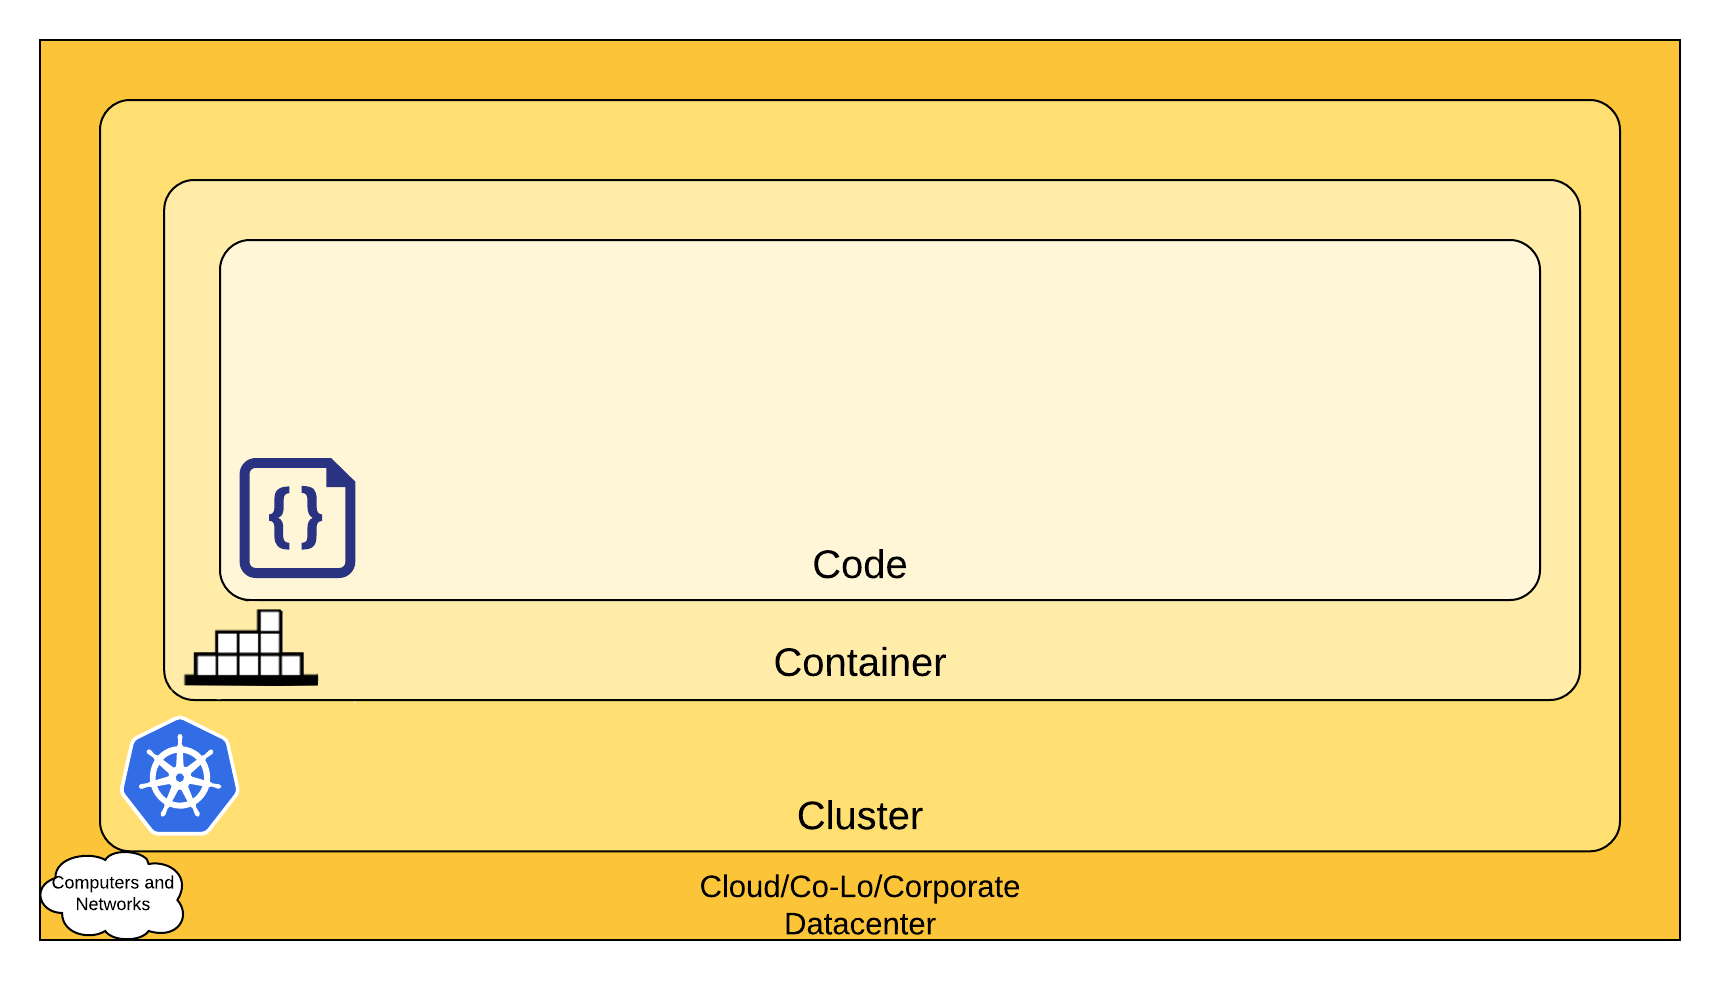
\includegraphics[width=0.4\textwidth]{images/cloud-security.png}
        \caption{Four layers of the cloud infrastructure.}
		\label{img:cloud-security}
	\end{center}
\end{figure}

Each layer is built upon the previous one and its security depends on the security of the outer layers. It is, therefore, important to maintain high security standarts on base levels (Cloud, Cluster, Container).

\begin{enumerate}

\item \textbf{Cloud} \\
Each cloud provider has its own security policies and guidelines. There are, however, some general infrastructure-level security best advice:

\begin{center}
    \begin{tabular}{ | m{16em} | m{16em} | } 
     \hline
     \textbf{Area of Concern for Kubernetes Infrastructure} & \textbf{Recommendation} \\ 
     \hline
     Network access to API Server (Control plane) & All access to the Kubernetes control plane is not allowed publicly on the internet and is controlled by network access control lists restricted to the set of IP addresses needed to administer the cluster. \\ 
     \hline
     Network access to Nodes (nodes)  & Nodes should be configured to only accept connections (via network access control lists) from the control plane on the specified ports, and accept connections for services in Kubernetes of type NodePort and LoadBalancer. If possible, these nodes should not be exposed on the public internet entirely. \\ 
     \hline
     Kubernetes access to Cloud Provider API & Each cloud provider needs to grant a different set of permissions to the Kubernetes control plane and nodes. It is best to provide the cluster with cloud provider access that follows the principle of least privilege for the resources it needs to administer. \\
     \hline
     Access to etcd & Access to etcd (the datastore of Kubernetes) should be limited to the control plane only. Depending on your configuration, you should attempt to use etcd over TLS. \\
     \hline
     etcd Encryption & Wherever possible it's a good practice to encrypt all storage at rest, and since etcd holds the state of the entire cluster (including Secrets) its disk should especially be encrypted at rest. \\
     \hline
    \end{tabular}
\end{center}

\item \textbf{Cluster} \\
There are two cluster security concerns that could be addressed: securing the configurable cluster components and securing the applications running in the cluster. Security of cluster components is described in **Cluster security** chapter.

There are a few things to consider regarding the application security:
\begin{itemize}
\item RBAC Authorization (Access to the Kubernetes API)
\item Authentication	
\item Application secrets management (and encrypting them in etcd at rest)
\item Ensuring that pods meet defined Pod Security Standards
\item Quality of Service (and Cluster resource management)
\item Network Policies
\item TLS for Kubernetes Ingress
\end{itemize}

\item \textbf{Container} \\
Securing containers is a vast topic, which deserves its own chapter. There are, nevertheless, a few general recommendation provided by the Kubernetes: 

\begin{center}
    \begin{tabular}{ | m{16em} | m{16em} | } 
     \hline
     \textbf{Area of Concern for Containers} & \textbf{Recommendation} \\ 
     \hline
     Container Vulnerability Scanning and OS Dependency Security & As part of an image build step, you should scan your containers for known vulnerabilities. \\ 
     \hline
     Image Signing and Enforcement & Sign container images to maintain a system of trust for the content of your containers. \\ 
     \hline
     Disallow privileged users & When constructing containers, create users inside of the containers that have the least level of operating system privilege necessary in order to carry out the goal of the container. \\
     \hline
    \end{tabular}
\end{center}

\item \textbf{Code} \\
When it comes to code, the developers have the most flexibility to design secure applications. There are a lot of issues to address, which may vary significantly from application to application depending on its purpose, architecture and framework base. Kubernetes documentation gives a handful of recommendations regarding this topic.

\begin{center}
    \begin{tabular}{ | m{16em} | m{16em} | } 
     \hline
     \textbf{Area of Concern for Code} & \textbf{Recommendation} \\ 
     \hline
     Access over TLS only & If your code needs to communicate by TCP, perform a TLS handshake with the client ahead of time. With the exception of a few cases, encrypt everything in transit. Going one step further, it's a good idea to encrypt network traffic between services. This can be done through a process known as mutual TLS authentication or mTLS which performs a two sided verification of communication between two certificate holding services. \\ 
     \hline
     Limiting port ranges of communication & This recommendation may be a bit self-explanatory, but wherever possible you should only expose the ports on your service that are absolutely essential for communication or metric gathering. \\ 
     \hline
     3rd Party Dependency Security & It is a good practice to regularly scan your application's third party libraries for known security vulnerabilities. Each programming language has a tool for performing this check automatically. \\
     \hline
     Static Code Analysis & Most languages provide a way for a snippet of code to be analyzed for any potentially unsafe coding practices. Whenever possible you should perform checks using automated tooling that can scan codebases for common security errors. \\
     \hline
     Dynamic probing attacks & There are a few automated tools that you can run against your service to try some of the well known service attacks. These include SQL injection, CSRF, and XSS. One of the most popular dynamic analysis tools is the OWASP Zed Attack proxy tool. \\
     \hline
    \end{tabular}
\end{center}   
                      
\end{enumerate}